\documentclass{acm_proc_article-sp}

\usepackage{algorithm}
%\usepackage{algorithmic}
\usepackage{algorithmicx}
\usepackage{algpseudocode}
\algrenewcommand\textproc{}
\usepackage{verbatim}
\usepackage{amssymb}

\begin{document}

\title{Improving Data Movement Performance by Balancing Network Load on the Blue Gene Q Supercomputer}

\numberofauthors{4}
\author{
% 1st. author
\alignauthor
Ben Trovato\\
       \affaddr{Institute for Clarity in Documentation}\\
       \affaddr{1932 Wallamaloo Lane}\\
       \affaddr{Wallamaloo, New Zealand}\\
       \email{trovato@corporation.com}
\and  % use '\and' if you need 'another row' of author names
% 4th. author
\alignauthor Lawrence P. Leipuner\\
       \affaddr{Brookhaven Laboratories}\\
       \affaddr{Brookhaven National Lab}\\
       \affaddr{P.O. Box 5000}\\
       \email{lleipuner@researchlabs.org}
\and
% 6th. author
\alignauthor Charles Palmer\\
       \affaddr{Palmer Research Laboratories}\\
       \affaddr{8600 Datapoint Drive}\\
       \affaddr{San Antonio, Texas 78229}\\
       \email{cpalmer@prl.com}
}

\maketitle
\begin{abstract}
Achievable networking performance in a supercomputer depends on the exact combination of communication patterns of applications and routing algorithms used by the supercomputer. However, while the communication patterns usually have wide spectrum and vary from application to applicaiton and phase to phase in an application, the routing algorithms have a limited variation and usually are optimized for typical communication patters. This results in high networking performance for favored communication patterns but low networking performance for other communication patterns. In this paper, we introduce approaches for improving networking performance by rebalancing load on physical links on the Blue Gene Q supercomputer. We realize our approaches into a framework called OPTIQ and demonstrate the efficacy of our framework via a set of benchmarks. The results show that we can achieve serveral times higher bandwidth than default mechannism MPI used in the Blue Gene Q supercomputer for certain communication patterns.
\end{abstract}

% A category with the (minimum) three required fields
%\category{H.4}{Information Systems Applications}{Miscellaneous}
%A category including the fourth, optional field follows...
%\category{D.2.8}{Software Engineering}{Metrics}[complexity measures, performance measures]

%\terms{Theory}

\keywords{data movement, load balancing, optimization, communication patterns} % NOT required for Proceedings

\section{Introduction}
\label{sec:intro}
Simulation time in a supercomputer depends partially in achievable networking performance in the supercomputer. The achievable networking performance in its turn depends on the exact combination of communication patterns of applications and routing algorithms used by the supercomputer. For each communication pattern there exists routing algorithms resulting in high networking performance. However, while the communication patterns have wide spectrum and vary time to time, the routing algorithms have a limited variation and usually are optimized for typical communication patters. This results in high networking performance for favored communication patterns but low networking performance for other communication patterns. Low networking performance subsequentially leads to long simulation time. Reducing the communication time for these non-favored communication pattern reduces the running time of an application. Thus, improving the networking performance for these communication patterns are important in redecing simulation time. 

Most of the routing algorithms are designed to perform well for certain communication patterns. However, for other communication patterns, they do not perform as well usually due to the unblanced on physically links caused by changing in the communication patterns. Rebalancing loads on the physical links in these situations can lead to better achievable performance. 
In this work, we propose a set of approaches that improve network performance for applications in supercomputers by rebalancing the load on physical links. Our approaches include using both heuristic algorithms and formal models with mathematical solvers to search for paths to move data from a set of sources to a set of destinations. The data then be divided into smaller messages and put into queues to move along found paths. The actual data movement can be done by using any available libraries for communication on the supercompter. We realize our approaches in a framework called OPTIQ. Our framework allows to easily expand the our work by adding algorithms for search paths, different way to schedule data transfer and different way to transfer data. It also allow to extend the framwork to other systems.

Our contributions include:
\begin{itemize}
\item Bring an insight understanding of how networking happens in the Blue Gene/Q supercomputer. By experiments, we show patterns that current routing algorithms favor and what it doesn not and explain why it happens it that way.
\item Propose a set of approaches to improve networking throughput by taking advantage of unused links or balancing network on links. We also explain when each approach should be used ot result highest possible throughputs.
\end{itemize}

Our paper includes the follows. In the next section, we present previous works in optimizing or improving data movement in various supercomputers or computing systems. In section \ref{sec:system}, we give a brief introduction to Mira - a Blue Gene Q supercomputer that we used to run our experiments. Section \ref{sec:approach} is the main section, where we explain about our framework and details of our approaches for each component of the framework. We demonstrate the efficacy of our approaches via a set of benchmarks in section \ref{sec:benchmark}. In section \ref{sec:conclusion}, we conclude our work and give some ideas about future work.


\section{Related work}
\label{sec:relatedwork}

Improving data movement performance by balancing network load has been studied in previous works. In \cite{Valiant81:Routing}, Valiant proposed a randomized routing mechanism mathematically proved to be able to route data globally with no sharing links for what network. However the routing mechanism did not work well in local routing \cite{singh2003:GOAL} . \cite{Pifarre91} proposed minimal routing optimization. However, it did not work well with global optimization \cite{singh2003:GOAL} . To address the limitation of both approaches, \cite{singh2003:GOAL} proposed GOAL – globally oblivious adaptive locally to balance load using adaptive routing algorithm for torus networks.

GOAL paper \cite{singh2003:GOAL}
Several bgq paper

\cite{Rodriguez09} proposed oblivious routing schemes in extended generalized fat tree networks. It extended 2 algorithms called S-mod-k and D-mod-k to provide a better oblivious solution for slimmed networks. 

\cite{Prisacari13a} showed that there is potential to optimize all-to-all collective exchange communication pattern at system level in fat tree networks and proved it mathematically and via simulations. The work is then extended in \cite{Prisacari13b} to propose a generic method to determine optimal pattern-specific routing for eXtended Generalized Fat Tree (XGFT). The method used a hybrid combination of integer linear programming (ILP) and dynamic programming. Interconnection network is divided into small subdomains and ILP is used for each subdomain. The local solution is then combined using dynamic programming. The proposed method takes up to several hours for several thousands of compute nodes interconnect network.

In other supercomputers, \cite{garcia2013:CrayDragonfly} proposed two deadlock-free routing mechanisms that support o
n-the-fly adaptive routing on Cray XC30 system for Dragonfly networks.

In Blue Gene Q, \cite{Chen:BGQ} proposed a heuristic routing for Blue Gene/Q supercomputing systems. The routing path is computed dynamically at the routing time based on coordinates of source and destination, partition shape and message size. The systems route a packet along the longest dimension of a partition first, shortest last. BG/Q systems route a message using single path. Different messages however might be routed using different paths.

Some optimizations are done based on system’s specific characteristics such as \cite{Kumar:Allreduce} proposed optimization for MPI\_Allreduce in BG/Q based on the observation on number links and other hardware supports on compute nodes.

Our previous works in \cite{Vishwanath:GLEAN} and \cite{SDAV:Bui2014b} addressed a problem of data aggregation for I/O purposes very dense in I/O case. In these works, we proposed . In a more recent work \cite{hbui:bgq} we presented our approaches for improving the performance very sparse. In this paper, we give solution for medium dense communication patterns between M and N.

In the next section, we briefly introduce Mira, a Blue Gene Q supercomputer that we used in our experiments in demonstrating the efficacy of our approaches.


\subsection{Experiment system}
\label{sec:system}

In this section, we describe Mira - an IBM Glue Gene Q supercomputer in which we developed our algorithms and a framework for network load balancing and conducted our experiments. Mira \cite{Chen:BGQ}, with 48 compute racks (48K nodes and 768K cores) at the ALCF, provides 10 PFlops theoretical peak performance. Each node has a 16-core processor and 16 GB of memory.

The interprocess communications of Blue Gene/Q travel on a 5D torus network both for point-to-point and for collective communications. This 5D torus interconnects a compute node with its 10 neighbors at 2 GB/s theoretical peak over each link in each direction, making a total of 40 GB/s bandwidth in both directions for a single compute node. Because of packet and protocol overheads, however, only up to 90\% of the raw data rate (1.8 GB/s) is available for user data. The machine can be partitioned into non-overlapping rectangular submachines; these submachines do not interfere with each other except for I/O nodes and the corresponding storage system.

For interconnect network traffic, BG/Q supports both deterministic and dynamic routing \cite{Chen:BGQ}. In deterministic routing, packets are routed based on dimension-ordered routing, from the longest first to the shortest last. In dynamic routing, routing is still dimension-ordered, but it is programmable, enabling different routing algorithms to be used. Given the size of a certain message, routing is always the same, and its path is known before it is routed. These are the default routing algorithms and cannot be changed during run time. However, one can set which routing zone id to use by using the PAMI\_ROUTING environment variable. Since BG/Q uses single-path data routing, for sending/receiving a message only one link of the ten available is used. The details of routing can be found in \cite{Chen:BGQ}.

PAMI is a low-level communication library for BG/Q \cite{PAMI:Kumar}. PAMI provides low-overhead communication by using various techniques such as accelerating communication using threads, scalable atomic primitives, and lockless algorithms to increase the messaging rate. Since MPI is implemented on top of PAMI, direct use of PAMI would provide higher messaging rates as well as lower latencies in comparison with MPI.




\section{Approaches}
\label{sec:approach}

In the Blue Gene Q supercomputers, data transfers are routed along using default routing algorithm. The default routing algorithm is proved to be well-balanced in many communication patterns \cite{Chen:BGQ}. However, for certain communication patterns, it results in poor performance due to unbalanced networking load on physical links. In this section, we present four approaches aiming for balancing load on physical links. We also give a brief description of a framework called OPTIQ, a realizationf of our approaches.

\subsection{Path searching approaches}
Four approaches that we present in this section include two heuristic algorithms, one multiple paths data movement taking advantages of existing shortest paths algorithms and one model-based approach. All paths searching algorihtms here are centric algorithms i.e. run at every node in exact order. Hence, every node has the same results. The approaches need some information in advance such as size, topology, torus of the partition, coordinates of all nodes in the partition. The information is collected once at the begining. The algorithms also need to have tuples of data movement requests: source, destination and amount of data to be transferred from the source to the destination.

\subsubsection{Heuristic 1}
In this approach, we search for paths between each pair of source and destination. From a source, we explore from all the destination in all possible directions. Whenever we reach a destination, we mark the destination as found to no longer search for it on other explorering paths from the same source. In this algorithm, we do not limit exploring paths by any constraints. The algorithm is described in \textbf{Algorithm \ref{alg:h1}}.

\begin{algorithm}
\textbf{Input:} Set of pairs of source-destination (\textit{s$_i$, d$_i$}). Number of nodes \textit{n}. Graph of nodes. \\
\textbf{Output:} Set of paths: one path for a pair of source-destination \\
\\
Structures:
\begin{algorithmic}
\State struct arc \{int u, int v\};
\State struct path \{set of arcs\};
\end{algorithmic}
Init:
    \begin{algorithmic}
	\State queue$<$struct path$>$ \textit{exploring\_paths} = $\varnothing$;
	\State queue$<$struct path$>$ \textit{complete\_paths} = $\varnothing$;
	\State bool \textit{visisted}[\textit{n}][\textit{n}];
	\For {0 $<=$ {\it i}, \textit{j} $<$ \textit{n}} 
	    \State \textit{visited}[{\it i}][{\it j}] = false;
	\EndFor
    \end{algorithmic}
Main:

\begin{algorithmic}
    \Function {Heuristic\_search\_I}{}

    \While {exist a source \textit{s$_i$} with unvisted neighbor \textit{u}}
	\State check\_and\_add\_new\_path({\it s}$_i$, \textit{u}, null);
	\State Pick next \textit{s$_i$} in the sources
    \EndWhile

    \While {(\textit{exploring\_path} != $\varnothing$)}
	\State path \textit{p} = \textit{exploring\_paths}.pop();
	\State {\it u} = last vertex in the path {\it p};
	\For {each neighbor \textit{v} of \textit{u}}
	    \State check\_and\_add\_new\_path({\it u}, \textit{v}, {\it p});
	\EndFor
    \EndWhile

    \EndFunction
\\
    \Function{check\_and\_add\_new\_path}{int \textit{u}, int \textit{v}, path {\it op}}
	\If {(!{\it visited}[{\it u}][{\it v}])}
	    \State create a path \textit{np} = {\it op}
	    \State add arc $<$\textit{u}, \textit{v}$>$ to \textit{np}
	    \State enqueue \textit{np} to \textit{exploring\_paths}
	    \If {{\it v} is one of the destinations of \textit{s$_i$} of \textit{np}}
	        \State enqueue \textit{np} to \textit{complete\_paths}
            \EndIf
	    \State {\it visited}[\textit{u}][\textit{v}] = true;
	\EndIf
    \EndFunction
\end{algorithmic}

\caption{Heuristic Alg 1: Exploring all paths without constraints}
\label{alg:h1}

\end{algorithm}

The \textbf{Algorithm \ref{alg:h1}} can be divided into 2 parts. In the first part, which is in the first \textbf{while} loop of the function Heuristic\_search\_I, we start at every source and add 1-hop paths to \textit{exploring\_paths} queue. Those paths are the paths from sources to their neighbors. We need a \textit{break} statement after each adding to make sure that every source can a path before they can all start again. This is to help ...

In the second part, which is the second \textbf{while} loop of the function Heuristic\_search\_I, we pop an exploring path \textit{p}from the \textit{exploring\_paths}. From the last added vertex \textit{u} of \textit{p}, we exploring all edges from it to it neighbors and add new path \textit{np} = \textit{p} + newly explored edge. If any of its neighbors is final destination of source \textit{s$_i$}, we then add \textit{np} into \textit{complete\_paths}. We continue the work until all the paths are explored.

Time complexity: The graph has V vertices and E edges. We have K pairs of (source, destinatinon), each source has at most D neighborhoods, then the time complexity of the \textbf{Algorithm \ref{alg:h1}} is $O$(K * (|V| + |E|)). The time complexity is breakdown as following:
\begin{itemize}
\item First part: we have K pairs hence K sources, for each source we discover its D neighbors, thus time will be $O$(K*D).
\item Second part: For this part, we get a path out of \textit{exploring\_paths}, create new paths by exploring its neighbors that are not visited by its source and add the new paths back to \textit{exploring\_paths}. For each sources, every vertex and every edge can be visited in the worst case, the time complexity would be $O$(|V| + |E|) minus to the vertices and edges visited by the first part. As we have K sources, the time complexity is $O$(K * (|V| + |E|)).
\end{itemize}

\subsubsection{Heuristic 2}
In the Algorithm \ref{alg:h1}, we explore all paths without concerning the number of hops that a path would take or maximum number of paths using a physical link. This leads to a long path or many paths sharing a physical link. A longer path results in more intermediate nodes, hence higher total transfer time. Higher maximum number of paths sharing a link leads to less bandwidth for each path. Both of them can lead to degraded performance.

This algorithm is an extension from Heuristic 1, in which we limit the exploring paths by both the number of hops and minimizing the maximum load. We do so by maintaining a min heap of paths. We use the heap to contain all the exploring paths instead of using a queue to manage the exploring paths as in Heuristic 1. This leads to increasing algorithm's time complexity in heap extracting (as taking data from a queue is O(1), from a min heap is O(log(n)) with n entries in the heap), but increasing the quality of explored paths. In this approach, we have finer results as we explore from least congested paths. The comparison function of the heap is based on both the number of hops and maximum load on each path. 

As most of the work in Heuristic 2 is similar to Heuristic 1, we do not repeat them, but only describe the differences between the two. The differences include:
\begin{itemize}
\item Use min heap of paths instead of queue of paths.
\item Need to heapify everytime we insert/delete from the min queue.
\end{itemize}

In the following, we describe the comparison function, which the core of the min heap for heapification. We also describe how to calculate the max load from the current load when adding a new path. We compare 2 paths based on its current max load and hop length. Among the two, max load has higher priority as max load affects the performance more.

\begin{algorithm}

Heap element comparison:
    \begin{algorithmic}
	\Function{heap\_compare} {path p1, path p2, int maxload, int maxhops}
	    \If {both paths has max load greater than maxload} 
		\State choose the one with smaller number of hops.
	    \EndIf
	    \If {One path has max load greater but one path has max load smaller than maxload}
		\State Choose the one with smaller load.
	    \EndIf
        \EndFunction
    \end{algorithmic}

\caption{Heuristic Alg 2: Exploring all paths with hops length and max load constraints}
\label{alg:h2}
\end{algorithm}

\subsubsection{Heuristic 3}

\begin{algorithm}
\textbf{Input:} Set of pairs of source-destination (\textit{s$_i$, d$_i$}). Number of nodes \textit{n}. Graph of nodes. Number of shortest path \textit{k}\\
\textbf{Output:} Set of paths: \textit{k} paths for a pair of source-destination\\
Init:
    \begin{algorithmic}
        \State queue$<$struct path$>$ \textit{complete\_paths};
    \end{algorithmic}
Main:
\begin{algorithmic}
    \Function {Heuristic\_search\_II}{}
	\For {each pair of source-dest (\textit{s$_i$}, \textit{s$_i$})}
	    \While{less than k paths discovered || still have paths to discover}
		\State Use Yen's algorithm to search for the shortest path \textit{p}.
		\State Check if adding \textit{p} make the current load over max load.
		\State If not, add \textit{p} into \textit{complete\_paths}
	    \EndWhile
	\EndFor
    \EndFunction
\end{algorithmic}

\caption{Heuristic Alg 3: k shortest paths}
\label{alg:h3}

\end{algorithm}

In the \textbf{Algorithm \ref{alg:h3}}, we use Yen's algorithm to search for k shortest paths between \textit{s$_i$, d$_i$}.

\begin{comment}

\subsubsection{Job-based AMPL model}
In this section we present a formal model written in A Modeling Language for Mathematical Programming (AMPL). The model captures demands of data movement between a set of sources and a set of destinations. The model also capture the graph of physical links of a partition given for the application. The model is presented in Model 1.

We presented the model in AMPL to solve the problem.

\begin{verbatim}
set Nodes;
set Arcs within Nodes cross Nodes;
set Jobs;

param Delay {Arcs} default 0;
param Capacity {Arcs} >= 0 default Infinity;
param Source {Jobs};
param Destination {Jobs} default 0;
param Demand {Jobs} default 0;

var Flow {Jobs, Arcs} >= 0;
var Z >= 0;

var total_flow{(i,j) in Arcs} = 
sum {job in Jobs} Flow[job,i,j];

maximize obj: Z;

subject to

zero_flow {job in Jobs, i in Nodes}:
sum{(i,j) in Arcs} Flow[job,i,j] - 
sum{(j,i) in Arcs} Flow[job,j,i] = 
if (i == Source[job])  then Demand[job]*Z 
else if (i == Destination[job]) then -Demand[job]*Z 
else 0;

capacity {(i,j) in Arcs}:
total_flow[i,j] <= Capacity[i,j];
\end{verbatim}

Model explanation:
\begin{itemize}
\item sets: we have 3 sets: \textit{Nodes}, \textit{Arcs} and \textit{Jobs}. \textit{JobID}: is the set of transfers from sources to destinations. Each job is represented by a tuple (id, source, destination, demand (total data size to transfer)).
\item params: {\it Delay}: delay on each arc; {\it Capacity}: capacity of each arc; {\it Source}: set of sources; {\it Destination}: set of destinations; {\it Demand}: amount of data to be transferred in each job.
\item vars: \textit{Flow}: total flow of each job on each arc; \textit{Z}: is reversed of total time; \textit{total\_flow} total flow of all jobs going through an arc.
\item objective function: we want to minimize the time or maximize its reversed value i.e. maximize \textit{Z}.
\item constraints(subject to): \textit{zero\_flow}: total flow through a source is total going out of that source, total flow going through a destination is total flow going in that destination, for other nodes that total is 0; \textit{capacity}: total flow on an arc is less than its capacity.
\end{itemize}

\end{comment}

\subsubsection{Path-based model}

\begingroup
\fontsize{9pt}{10pt}\selectfont

\begin{verbatim}
set Nodes;
set Arcs within Nodes cross Nodes;
# Origin/Destination pairs
set OD within Nodes cross Nodes;
set Paths{OD};
set Path_Arcs{od in OD, p in Paths[od]}
    within Arcs;


param Capacity {Arcs} >= 0 default Infinity;
param Demand {OD} default 0;

var Flow {Paths} >= 0;
var Z >= 0;

var total_flow{(i,j) in Arcs} = 
    sum {p in Paths} Flow[job,i,j];

maximize obj: Z;

subject to

zero_flow {p in Paths, i in Nodes}:
sum{(i,j) in Arcs} Flow[job,i,j] - 
    sum{(j,i) in Arcs} Flow[job,j,i] =
    if (i == Source[job]) then Demand[job]*Z else 
    if (i == Destination[job]) then -Demand[job]*Z 
    else 0;

capacity {(i,j) in Arcs}:
total_flow[i,j] <= Capacity[i,j];
\end{verbatim}

\endgroup

Model explanation:
\begin{itemize}
\item sets: we have 5 sets: \textit{Nodes}, \textit{Arcs}, \textit{OD}, \textit{Paths} and \textit{Path\_Arcs}. \textit{JobID}: is the set of transfers from sources to destinations. Each job is represented by a tuple (id, source, destination, demand (total data size to transfer)).
\item params: {\it Capacity}: capacity of each arc; {\it Demand}: amount of data to be transferred in each job between a pair of orgin and destination.
\item vars: \textit{Flow}: total flow of each job on each arc; \textit{Z}: is reversed of total time; \textit{total\_flow} total flow of all jobs going through an arc.
\item objective function: we want to minimize the time or maximize its reversed value i.e. maximize \textit{Z}.
\item constraints(subject to): \textit{zero\_flow}: total flow through a source is total going out of that source, total flow going through a destination is total flow going in that destination, for other nodes that total is 0; \textit{capacity}: total flow on an arc is less than its capacity.
\end{itemize}

So far, we have presented different algorithms/approaches: here is when to use what:

\begin{table}[h]
\begin{center}
    \begin{tabular}{ | p{1.6cm} | l | p{3cm} |}
    \hline
    Approach & Time complexity & When to use \\ \hline
    Heuristic 1 & $O$(K * (|V| + |E|)) &  Used as first step for Heuristic 2\\ \hline
    Heuristic 2 & $O$(K * (|V| + |E|)) &  Very dense communication\\ \hline
    Heuristic 3 & $O$(K * (|V| + |E|)) & Sparse comminication \\ \hline
    Path-based model & $O$(K * (|V| + |E|)) & Medium dense where proportional throughtput can be gained \\
    \hline
    \end{tabular}

    \caption{Approaches: time complexity and usage}
    \label{tbl:experiment}

\end{center}
\end{table}

We realize algoirthms and other work in a framework named OPTIQ. The framework provides ways to improve data movement performance on the Blue Gene/Q supercomputer. Our framework does so by balancing loads on physical links on the Blue Gene/Q supercomputer.

\subsection{Framework}

Our framework has 3 main components: Path searching algorithms, Schedule and Transport and an extra component depicted in Figure \ref{fig:framework}.

\begin{figure}[!htb]
\vspace{-0.1in}
\centering
\includegraphics[scale=0.7]{figures/framework.pdf}
\vspace{-0.2in}
\caption{Three components of OPTIQ framework}
\vspace{-0.1in}
\label{fig:framework}
\end{figure}

The functionarity of each component is as following:
\begin{itemize}
\item Path searching: search for path to transfer data from a set of sources to a set of destination. Multiple or single paths can be found using a set of algorithm. User can decide what algorithm to be used or let the framework use a default algorithm.
\item Schedule: Split a buffer data that needed to tranfer into smaller messages and put those messages into a queue of transport layer to be transferred. It also handles incoming messages for itself and for forwardig them to its neighbors on a way to a message final destination.
As we route data in our own ways, we search for the paths, and we also need to schedule messages transfer. It includes sending local messages, forwarding messages form other sources, receiving data as the intermediate node or the destination node.

Order of messages into sending queue: 3 types of messages: local messages (needed to send), fowarding messages (needed to send), its receiving messages. first come first serve, local messages first. forwa

When there are multiple ranks per node, which one will be choosen to receive data at the next dest (forwarding). Single rank to do or many rank to do, currently every rank executes data transfer.

\item Transport: actually transfer an amount of data from one point to another point in the system.
\item Extra component: To get system specific information such as partition size, topology, coordinates, torus, and to compute neighbors of available nodes given to an application. Topology reading, coord, neighbors, torus, size, routing order, graph generated. Also set of benchmarks, tests.

the framework allow various options that allow to do: forwarding/local message sending order, algorithm selection, chunk size, transport implementations...
\end{itemize}


\section{Experiments and Results}
\label{sec:benchmark}

In this section, we demonstrate the efficacy of our approaches through multiple experiments on a leadership-scale system. We describe the system, the implementation details, the experimental setup and present the results in the following sections.
%via a set of benchmarks. Our experiments were carried on Mira, a Blue Gene/Q supercomputer. We give a brief description of the supercomputer before presenting and analysing our experiments and results.

\subsection{Experiment system}
\label{sec:system}

In this section, we describe Mira - an IBM Glue Gene Q supercomputer in which we developed our algorithms and a framework for network load balancing and conducted our experiments. Mira \cite{Chen:BGQ}, with 48 compute racks (48K nodes and 768K cores) at the ALCF, provides 10 PFlops theoretical peak performance. Each node has a 16-core processor and 16 GB of memory.

The interprocess communications of Blue Gene/Q travel on a 5D torus network both for point-to-point and for collective communications. This 5D torus interconnects a compute node with its 10 neighbors at 2 GB/s theoretical peak over each link in each direction, making a total of 40 GB/s bandwidth in both directions for a single compute node. Because of packet and protocol overheads, however, only up to 90\% of the raw data rate (1.8 GB/s) is available for user data. The machine can be partitioned into non-overlapping rectangular submachines; these submachines do not interfere with each other except for I/O nodes and the corresponding storage system.

For interconnect network traffic, BG/Q supports both deterministic and dynamic routing \cite{Chen:BGQ}. In deterministic routing, packets are routed based on dimension-ordered routing, from the longest first to the shortest last. In dynamic routing, routing is still dimension-ordered, but it is programmable, enabling different routing algorithms to be used. Given the size of a certain message, routing is always the same, and its path is known before it is routed. These are the default routing algorithms and cannot be changed during run time. However, one can set which routing zone id to use by using the PAMI\_ROUTING environment variable. Since BG/Q uses single-path data routing, for sending/receiving a message only one link of the ten available is used. The details of routing can be found in \cite{Chen:BGQ}.

PAMI is a low-level communication library for BG/Q \cite{PAMI:Kumar}. PAMI provides low-overhead communication by using various techniques such as accelerating communication using threads, scalable atomic primitives, and lockless algorithms to increase the messaging rate. Since MPI is implemented on top of PAMI, direct use of PAMI would provide higher messaging rates as well as lower latencies in comparison with MPI.



\subsection{Implementation Details}

PAMI is a low-level communication library for BG/Q \cite{PAMI:Kumar}. PAMI provides low-overhead communication by using various techniques such as accelerating communication using threads, scalable atomic primitives, and lockless algorithms to increase the messaging rate. Since MPI is implemented on top of PAMI, direct use of PAMI would provide higher messaging rates as well as lower latencies in comparison with MPI. We used PAMI\_Put for large messages and PAMI\_Send\_immediate for control messages.


\subsection{Experiment setup}

We carried our experiments on Mira, a Blue Gene/Q supercomputer. In our experiments, we varied paritition size from 512 nodes up to 8012 nodes. The experiments involved a subset or entire set of nodes for each partition. The number sources and destinations and distance between them are also varied depending on each experiment. We also varied the data sizes to be exchanged to find the effective data size. Pairs of sources and destinations are randomized to show the efficacy of our works. We varied the number of paths fed into solvers to measure the effectiveness of number of paths to throughput. A similar benchmark with various max load is done for heuristic approach. Our experiments covered 3 communication patterns: Disjoint, Overlap and Subset. For the commnication patterns, we demonstrated the efficacy of our algorithms in comparions with MPI\_Alltoallv.

For searching optimal paths, we used AMPL (A Modeling Language for Mathematical Programming) and its solvers \cite{AMPL} for modeling our problem and to find solutions for optimal data movement.

We demonstrate the data movement performance of our OPTIQ framework and existing MPI routines on three communication patterns -- {\em disjoint}, {\em overlap} and {\em subset}, illustrated in Figure \ref{fig:patterns}. In this figure, m and n refer to set of source or destination nodes. These patterns are owing to different possible relationships between source and destination nodes as described below:
\begin{itemize}
\item Disjoint: There are distinct sources and destinations. It is a common data movement pattern present in many applications.
\item Overlap: The sources and destinations are overlapped sets. Some applications like CESM uses this communication pattern for coupling.
\item Subset: Either the set of source nodes is subset of the destination nodes or vice versa. This pattern can be found in CESM and in collective I/O aggregation phase.
\end{itemize}
\begin{figure}[ht]
\vspace{-0.15in}
\centering
\includegraphics[scale=0.48]{figures/patterns.pdf}
\vspace{-0.15in}
\caption{\small Communication patterns}
\vspace{-0.15in}
\label{fig:patterns}
\end{figure}

We demonstrate throughput improvement in a complex network like 5D torus through the above diverse communication patterns. We compare the efficacy of our algorithms with MPI\_Alltoallv, which is the most commonly used MPI collective for the data movement patterns considered in our work.

%\subsection{MPI path reconstruction}

We measure several network-related metrics such as load on physical links, and the number of hops per data-transfer path, for the above benchmarks, using our approaches and MPI\_Alltoallv. The load and number of hops highlight performance differences between MPI and OPTIQ. The performance metrics are output directly in case of OPTIQ. However, MPI\_Alltoallv does not output all of these performance metrics. Thus, we need to reconstruct the data-transfer paths taken by MPI collectives. We reconstruct the paths based on the routing algorithms described in \cite{Chen:BGQ}. For each pair of source and destination nodes, we start at a source node and trace the route taken by the MPI message according to the rules of the routing algorithm. We record paths for all source-destination pairs and use this information to calculate load and number of hops for MPI\_Alltoallv. 

%In our experiment we need to measure not only the performance of MPI routines, but also loads on physical links, and the number of hops per path that MPI takes to move data from a set of sources to a set of destination. The load and hops information can reveal details on performance differences between MPI and our framework OPTIQ. Thus reconstructing MPI's paths is necessary to get load and hops information.
%We reconstruct MPI's paths based on our understanding of default routing algorithms described in \cite{Chen:BGQ}. For each pair of source and destination we start at a source node and follow the rules of the routing algorithm to move data from the source node to its destination. We then record paths for all the pairs and use them to calculate load and number of hops.


\subsection{Results}
\label{sec:results}

We measured throughput, total number of paths, maximum and average values for number of paths per job, hopbytes (total bytes $\times$ number of hops) per path, number of copies per paths, number of paths per link, and total amount of data per link for various communication patterns, source destination pairing, distance and sizes of sources and destinations, partition sizes, message sizes, and chunk size. In the next subsections, we present our results and detailed study of system behaviour and network performance for our benchmarks.
%go into each communication and study in detail the system's behaviors and performance.

\subsubsection{Varying partition, source and destination sizes, keeping the same source to destination ratio}

In this experiment we vary the number of sources and destinations, together with total number of nodes, while keeping a constant ratio of 1:8 between the number of sources and destination nodes. We increase the total number of nodes P from 512 to 4096, The first P/16 nodes send data to the last P/2 nodes. Each source has 8 destinations e.g. node 0 sends data to nodes P/2, P/2+1, ... P/2+7. We present results for {\em disjoint}, {\em overlap} and {\em subset} communications using OPTIQ Optimization (OPT), OPTIQ Heuristic (HEU) and MPI\_Alltoallv (MPI). We use 1 MPI/PAMI rank/node. The data size is 8 MB per source-destination pair. 
%We set the $maxload$ to 16 for the Heuristic approach. %already mentioned 

Figure \ref{fig:constantr} shows the throughput for OPT, HEU and MPI. As shown in the figure, the Optimization approach has the highest throughput, followed by the Heuristic approach and MPI\_Alltoallv. This is because OPT and HEU uses multiple paths for data transfer. Additionally, OPT globally balances load for all source-destination pairs. %TODO: We see improved throughput for 4096 nodes in the case of OPT and HEU because ..... data / hopbytes for 512 vs 4096 performance.  

\begin{figure*}[!htbp]
        \centering
        \begin{subfigure}[b]{0.32\textwidth}
                \includegraphics[width=\textwidth]{figures/constantr_3.pdf}
                \caption{Disjoint}
                \label{fig:constantr_3}
        \end{subfigure}%
        ~ %add desired spacing between images, e. g. ~, \quad, \qquad, \hfill etc.
          %(or a blank line to force the subfigure onto a new line)
        \begin{subfigure}[b]{0.32\textwidth}
                \includegraphics[width=\textwidth]{figures/constantr_27}
                \caption{Overlap}
                \label{fig:constantr_27}
        \end{subfigure}
        ~ %add desired spacing between images, e. g. ~, \quad, \qquad, \hfill etc.
          %(or a blank line to force the subfigure onto a new line)
        \begin{subfigure}[b]{0.32\textwidth}
                \includegraphics[width=\textwidth]{figures/constantr_87}
                \caption{Subset}
                \label{fig:constantr_87}
        \end{subfigure}
        \caption{\small Varying the number of sources and destinations and total number of nodes while keeping the ratio constant (1:8).}
	\vspace{-0.15in}
        \label{fig:constantr}
\end{figure*}

Table \ref{table:constantr} shows the throughput, total number of paths per job, the hopbytes per path, the number of copies per path, number of paths per physical link and the total data per link for 1024 nodes. In all three cases, our greedy heuristic is able to find the highest number of paths for the entire data flow. HEU also has the highest maximum and average number of paths per job. However, the paths found by Heuristic are based on local optimization of load on the physical links, as explained in Section~\ref{sec:heuristic}. Therefore, there are higher number of paths per physical link, and higher amount of data per physical link in HEU as compared to OPT. OPT has lower number of paths per link because OPT globally load balances the data transfer on physical links.
%TODO: table remove columns
\begin{comment}
\begin{table*}[!htbp]
   \centering
    \begin{tabular}{| p{0.5cm} | l | r | r | p{0.5cm} | p{0.5cm} | p{0.5cm} | p{0.5cm} |p{0.4cm} | p{0.5cm} |p{0.4cm} | p{0.4cm} |p{0.50cm} | p{0.6cm} |}
    \hline
    \multirow{3}{*}{Pattern} & \multirow{3}{*}{Type} & \multirow{3}{1cm}{nW (GB/s)} & \multicolumn{3}{ c| }{Num. of Paths} & \multicolumn{2}{ c| }{Hopbytes} & \multicolumn{2}{ c| }{Num of copies}& \multicolumn{2}{ c| }{Num of paths} & \multicolumn{2}{ c| }{Total data} \\ \cline{4-6}
    & & & \multirow{2}{0.5cm}{Total Paths} & \multicolumn{2}{ c| }{Per Job} & \multicolumn{2}{ c| }{Per Path (MB)} & \multicolumn{2}{ c| }{Per Path}& \multicolumn{2}{ c| }{Per Link}& \multicolumn{2}{ c| }{Per Link (MB)} \\ \cline{5-14}
    & & & & {Max} & Avg & Max & Avg & Max & Avg & Max & Avg & Max & Avg\\ \hline
    \multirow{3}{*}{Disjoint} & OPT    & 188.62 & 1169 & 6 & 2.28 & 83.88 & 23.02 & 1152 & 295.22 & 11 & 2.53 & 18.28 & 9.26 \\ \cline{2-14}
    & HEU & 74.88  & 3146 & 23 & 6.14 & 83.88 & 8.45 & 1152 & 108.24 & 16 & 4.94 & 63.04 & 6.92 \\ \cline{2-14}
    & MPI    & 45.18  & 512  & 1 & 1.00 & 92.27 & 50.33 & & & 16 & 3.07 & 134.21 & 25.76\\ \hline
    \multirow{3}{*}{Overlap} & OPT    & 200.03 & 1303 & 6 & 2.54 & 83.88 & 19.28  & 1152 & 243.96 & 13 & 2.74 & 16.97 & 9.04\\ \cline{2-14}
    & HEU & 113.17  & 3273 & 26 & 6.39 & 75.49 & 7.41 & 1024 & 93.07 & 16 & 5.17 & 38.66 & 7.04 \\ \cline{2-14}
    & MPI    & 42.84 & 512 & 1 & 1.00 & 83.88 & 42.99 &  & & 16 & 3.38 & 134.21 & 28.36 \\ \hline
    \multirow{3}{*}{Subset} & OPT    & 199.20 & 1269 & 6 & 2.48 & 75.49 & 19.48 & 1024 & 245.66 & 11 & 2.79 & 17.10 & 9.32 \\ \cline{2-14}
    & HEU &  61.71 & 3238 & 26 & 6.32 & 75.49 & 7.43 & 1024 & 93.22 & 16 & 5.28 & 45.08  & 7.35 \\ \cline{2-14}
    & MPI    &  41.37 & 512  & 1 & 1.00 & 83.88 &  41.94 & & & 16 & 3.52 & 134.21 & 29.49 \\ \hline
    \end{tabular}
    \caption{\small Throughput, total number of paths, number of paths per job, maximum and average values of hopbytes, number of copies, number of paths per link and amount of data per link for 3 patterns in 1024 nodes experiments.}
    \label{table:constantr}
\end{table*}
\end{comment}

\begin{table}[!htbp]
   \centering
    \begin{tabular}{| L{0.65cm} | L{0.4cm} | R{0.6cm} | R{0.5cm} | R{0.3cm} | R{0.4cm} | R{0.4cm} | R{0.3cm} | R{0.90cm} |}
    \hline
    \multirow{3}{*}{Pattern} & \multirow{3}{*}{Type} & \multirow{3}{0.6cm}{BW (GB/s)} & \multicolumn{3}{ c| }{Num. of Paths} & \multicolumn{2}{ c| }{Num of paths} & \multirow{3}{1.15cm}{Max amt. of data / link (MB)} \\ \cline{4-6}
    & & & \multirow{2}{0.5cm}{Total Paths} & \multicolumn{2}{ c| }{Per Job} & \multicolumn{2}{ c| }{Per Link}& \\ \cline{5-8}
    & & & & {Max} & Avg & Max & Avg & \\ \hline
    \multirow{3}{*}{Disjoint} & OPT    & 188.62 & 1169 & 6 & 2.28 & 11 & 2.53 & 18.28 \\ \cline{2-9}
    & HEU & 74.88  & 3146 & 23 & 6.14 & 16 & 4.94 & 63.04 \\ \cline{2-9}
    & MPI    & 45.18  & 512  & 1 & 1.00 & 16 & 3.07 & 134.21 \\ \hline
    \multirow{3}{*}{Overlap} & OPT    & 200.03 & 1303 & 6 & 2.54 & 13 & 2.74 & 16.97 \\ \cline{2-9}
    & HEU & 113.17  & 3273 & 26 & 6.39 & 16 & 5.17 & 38.66 \\ \cline{2-9}
    & MPI    & 42.84 & 512 & 1 & 1.00 & 16 & 3.38 & 134.21 \\ \hline
    \multirow{3}{*}{Subset} & OPT    & 199.20 & 1269 & 6 & 2.48 & 11 & 2.79 & 17.10 \\ \cline{2-9}
    & HEU &  61.71 & 3238 & 26 & 6.32 & 16 & 5.28 & 45.08 \\ \cline{2-9}
    & MPI    &  41.37 & 512  & 1 & 1.00 & 16 & 3.52 & 134.21 \\ \hline
    \end{tabular}
    \caption{\small Throughput, total number of paths, number of paths per job, maximum and average values number of paths per link and max amount of data per link for 3 patterns in 1024 nodes experiments.}
    \vspace{-0.15in}
    \label{table:constantr}
\end{table}

Figure \ref{fig:loaddata_histo} shows the distribution of data per link for OPT, HEU and MPI. Optimization approach considers the global load on the network and hence data is distributed among the paths in a more balanced way such that the physical links are load-balanced. Thus, OPT has the lowest maximum amount of data per physical link as shown in Figure \ref{fig:loaddata_histo}. MPI\_Alltoallv has the lowest number of paths. With 1 path per pair of communication, entire data is transferred using the single path, without utilizing the other idle links. %Thus it has the highest hopbytes per path as can be observed in Figure \ref{fig:hopbyte_histo}. 
MPI has the highest amount of data per physical link as can be observed in Figure \ref{fig:loaddata_histo}. Thus MPI has the lowest throughput.
\begin{figure}[!htb]
\vspace{-0.15in}
\centering
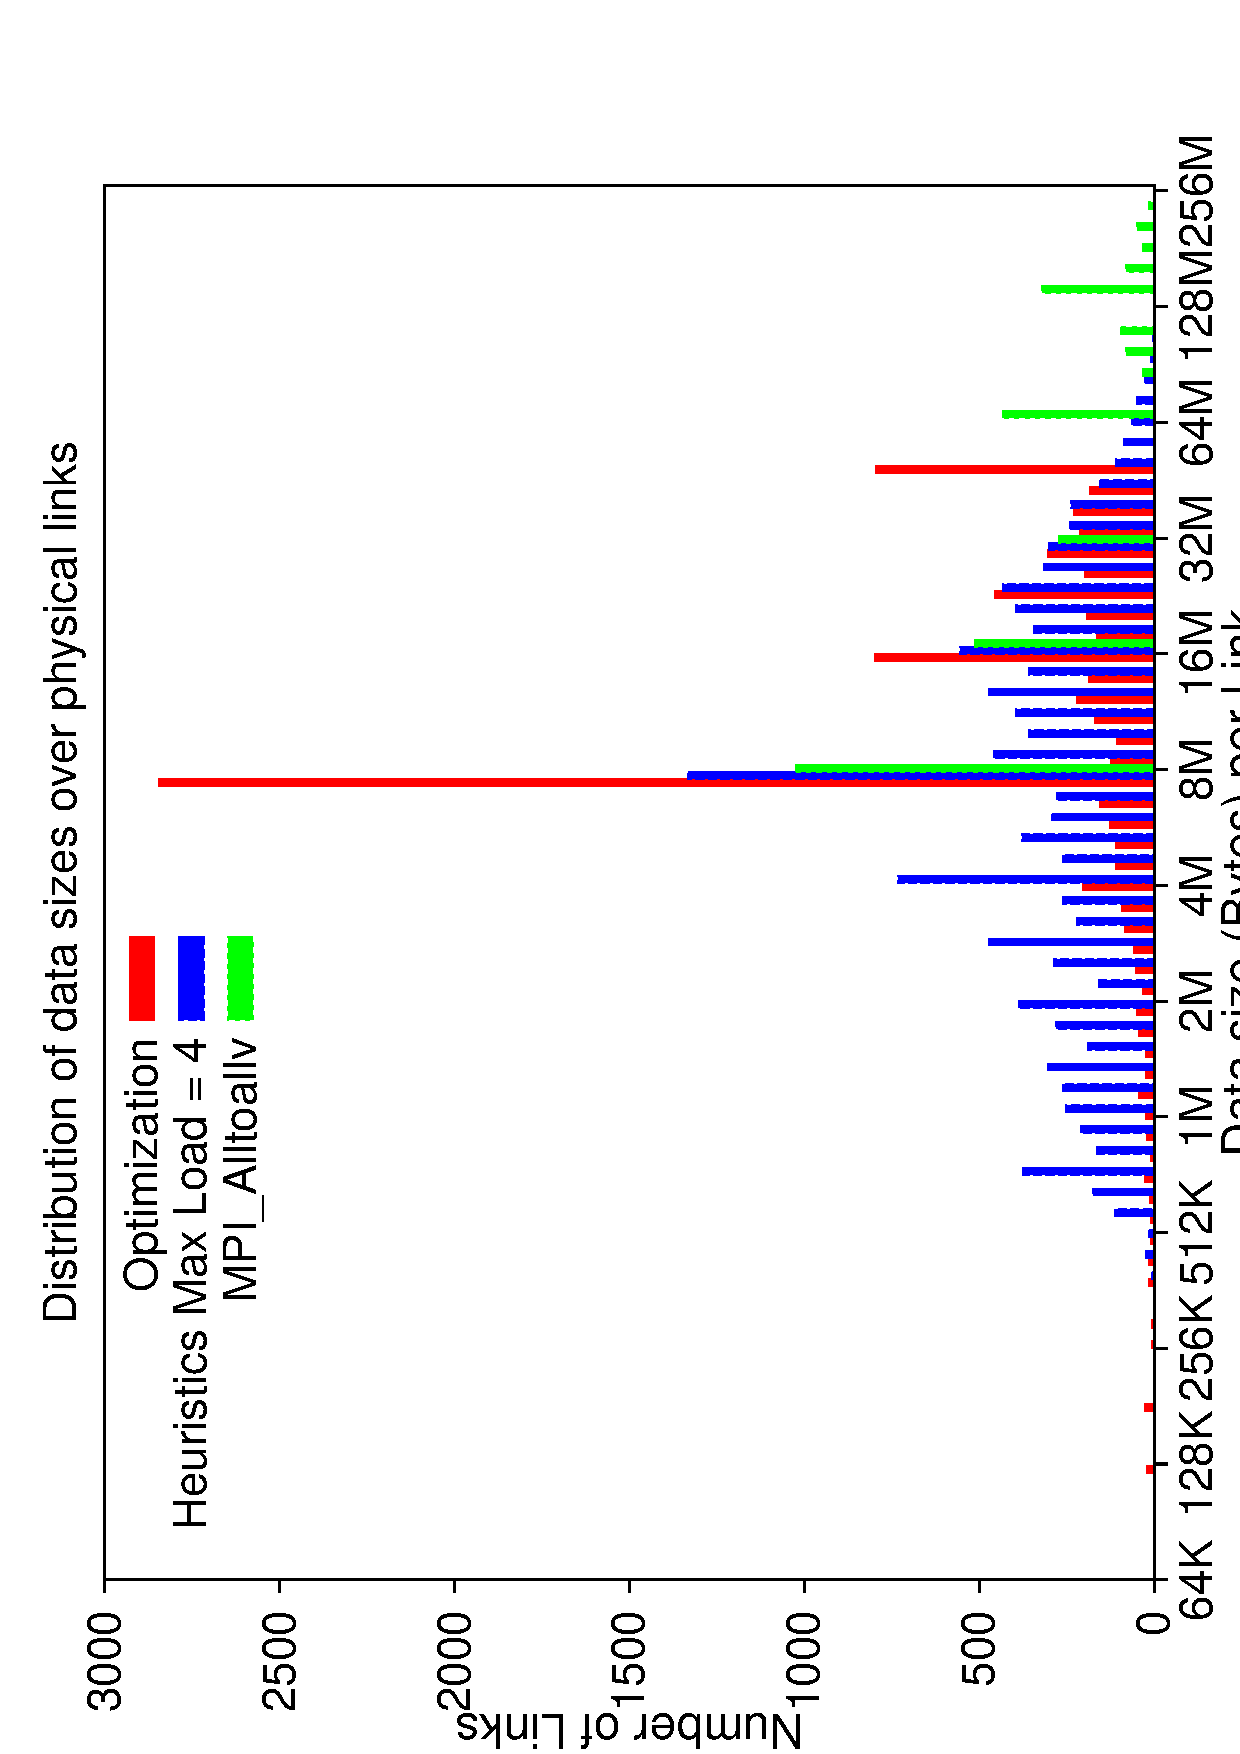
\includegraphics[scale=0.27]{figures/loaddata_histo.pdf}
\vspace{-0.15in}
\caption{\small Distribution of total amount of data per link for Disjoint pattern in 1024-node partition.}
\vspace{-0.15in}
\label{fig:loaddata_histo}
\end{figure}

%\begin{figure}[!htb]
%\vspace{-0.1in}
%\centering
%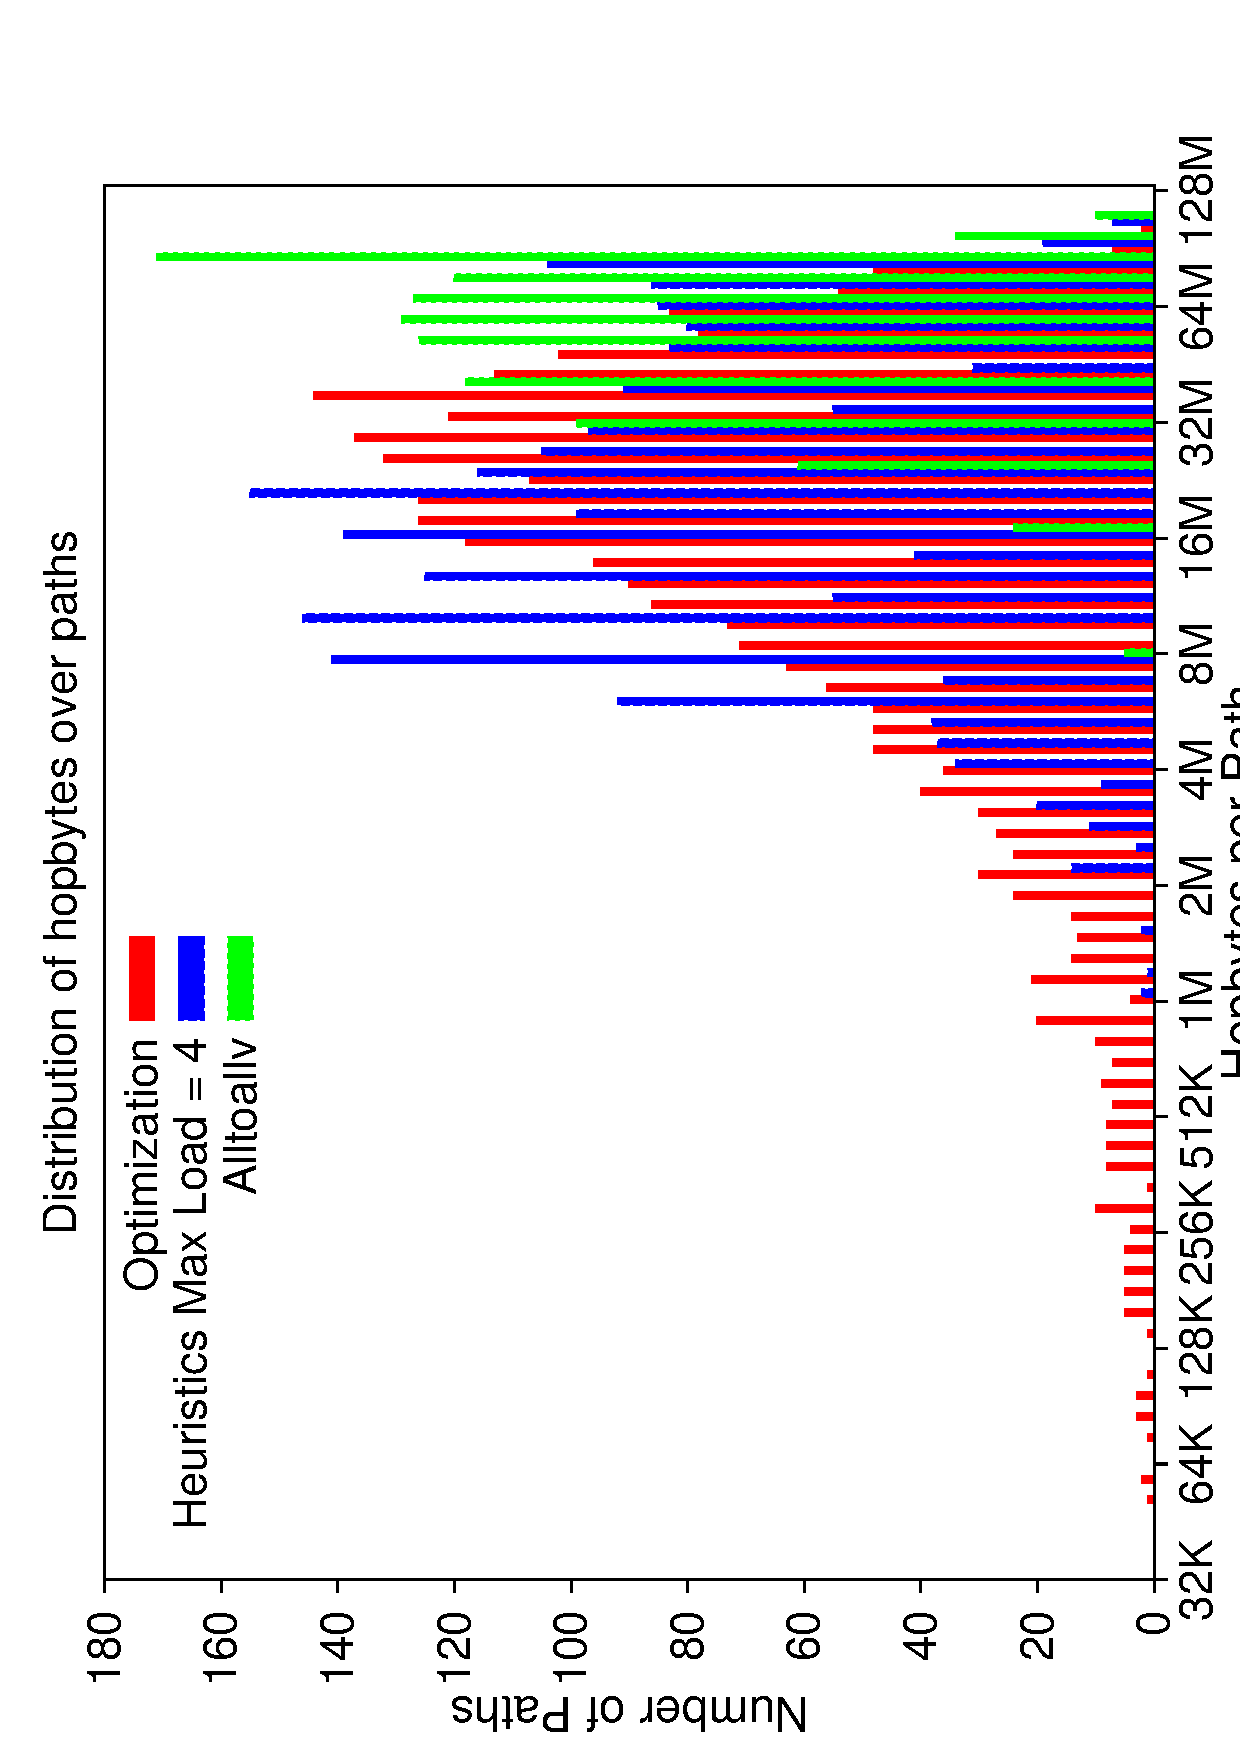
\includegraphics[scale=0.30]{figures/hopbyte_histo.pdf}
%\vspace{-0.1in}
%\caption{Distribution of hopbytes per path for Disjoint pattern in 1024-node partition.}
%\vspace{-0.1in}
%\label{fig:hopbyte_histo}
%\end{figure}




\subsubsection{Increasing distance between source and destination nodes}

Figure ~\ref{fig:incrdist} shows the throughput of OPTIQ Optimization (OPT), OPTIQ Heuristic (HEU), and MPI\_Alltoallv (MPI) for disjoint, overlap and subset configurations. The experiment was done in a 2048-node partition with 256 source nodes communicating to 512 destination nodes. The set of destination nodes is chosen such that the average distance between source and destination nodes increases. Distance between 2 nodes implies the number of hops between them. The x-axes in Figures \ref{fig:incrdist_disjoint}, \ref{fig:incrdist_overlap} and \ref{fig:incrdist_subset} represent the different destination node positions. For example, in Figure \ref{fig:incrdist_disjoint}, the sources are from 0--255 and the destination position 1 refer to destination node set from node 256--767, position 2 refers to node 512--1023, position 3 refers to node 1024--1535, and destination position 4 refers to 1536--2047. The y-axes shows the throughput. We observe that the throughput of OPT and HEU increases with increasing distance in case of disjoint. This is because OPT and HEU are able to find more paths with increasing distance without increasing the maximum load on the physical links. Both Optimization and Heuristics approaches outperform MPI\_Alltoallv which uses single path for communication.
%location is moving to increase the number of hops between sources and destinations. In this experiment we show that when the distance between set of source nodes and set of destination nodes increases, we are able to find more paths while not increasing the maximum load on the physical links, thus improving performance. 
\begin{figure*}[!htbp]
        \centering
        \begin{subfigure}[b]{0.32\textwidth}
                \includegraphics[width=\textwidth]{figures/incrdist_disjoint.pdf}
                \caption{Disjoint}
                \label{fig:incrdist_disjoint}
        \end{subfigure}%
        ~ %add desired spacing between images, e. g. ~, \quad, \qquad, \hfill etc.
          %(or a blank line to force the subfigure onto a new line)
        \begin{subfigure}[b]{0.32\textwidth}
                \includegraphics[width=\textwidth]{figures/incrdist_overlap}
                \caption{Overlap}
                \label{fig:incrdist_overlap}
        \end{subfigure}
        ~ %add desired spacing between images, e. g. ~, \quad, \qquad, \hfill etc.
          %(or a blank line to force the subfigure onto a new line)
        \begin{subfigure}[b]{0.32\textwidth}
                \includegraphics[width=\textwidth]{figures/incrdist_subset}
                \caption{Subset}
                \label{fig:incrdist_subset}
        \end{subfigure}
        \caption{Total data movement throughput with increasing distance between sources and destinations.}
        \label{fig:incrdist}
\end{figure*}

\begin{table*}%[!htbp]
   \centering
    \begin{tabular}{| p{0.85cm} | p{0.5cm} | p{0.5cm} | p{0.6cm} | p{0.6cm} | p{0.5cm} | p{0.5cm} |p{0.6cm} | p{0.6cm} | p{0.5cm} | p{0.5cm} |p{0.6cm} | p{0.6cm} |p{0.5cm} | p{0.5cm} |p{0.6cm} | p{0.6cm} |}
    \hline
     Positions & \multicolumn{4}{ c | }{1} & \multicolumn{4}{ c| }{2} & \multicolumn{4}{ c| }{3} & \multicolumn{4}{ c| }{4} \\ \hline
     Patterns & {Max distance} & {Avg distance} & OPT \#Paths & HEU \#Paths & Max distance & Avg distance & OPT \#Paths & HEU \#Paths & Max distance & Avg distance & OPT \#Paths & HEU \#Paths & Max distance & Avg distance & OPT \#Paths & HEU \#Paths \\ \hline
     Disjoint & 14 & 7.50 & 1105 & 2822 & 14  & 7.50 & 1372 & 2887 & 15 & 8.50 & 1547 & 3668 & 15 & 8.50 & 1672 & 3834 \\ \hline
     Overlap & 13 & 7.25 & 2085 & 6460 & 14  & 7.69 & 2152 & 3671 & 15 & 7.88 & 2337 & 6548 & 18 & 9.59 & 2399 & 7010 \\ \hline
     Subset &  20 & 8.56 & 1840 & 3422 & 21  & 8.56 & 1639 & 3364 & 22 & 9.06 & 1594 & 3119 & 23 & 9.06 & 1477 & 3087 \\ \hline
    \end{tabular}
    \caption{Maximum (Max) and average (Avg) distance between sources and destinations and number of paths for OPT and HEU for {\em disjoint}, {\em overlap} and {\em subset} on 2048 Mira nodes.}
    %\caption{Maximum (Max) and average (Avg) distance and number of paths between sources and destinations at each position.}
    \label{table:incrdist}
\end{table*}

Table \ref{table:incrdist} shows the corresponding maximum and average distances between source and destination nodes, and the number of paths for OPT and HEU for the configurations in Figure \ref{fig:incrdist}. Number of paths for MPI is 512. In general, performance of OPT improves with higher number of paths as seen in the first row for disjoint. It can also be seen that the number of paths decreases for OPT in the case of subset which leads to decrease in throughput. HEU has more paths than OPT but due to imbalanced data distribution, throughput of HEU is lower than OPT.  
%The number of paths produced by Optimization approach are 1105, 1372, 1547 and 1672 respectively. With increasing number of paths, the hopbytes, number of copies per paths and data load per physical link decrease, thus increasing in performance as shown in Figure \ref{fig:incrdist}. The same trend is observed in the Heuristics approach.


\subsubsection{Increasing number of destination nodes}
\label{sec:incrdestnodes}

\begin{figure*}%[!htbp]
        \centering
        \begin{subfigure}[b]{0.32\textwidth}
                \includegraphics[width=\textwidth]{figures/incrsize_disjoint.pdf}
                \caption{Disjoint}
                \label{fig:incrsize_disjoint}
        \end{subfigure}%
        ~ %add desired spacing between images, e. g. ~, \quad, \qquad, \hfill etc.
          %(or a blank line to force the subfigure onto a new line)
        \begin{subfigure}[b]{0.32\textwidth}
                \includegraphics[width=\textwidth]{figures/incrsize_overlap}
                \caption{Overlap}
                \label{fig:incrsize_overlap}
        \end{subfigure}
        ~ %add desired spacing between images, e. g. ~, \quad, \qquad, \hfill etc.
          %(or a blank line to force the subfigure onto a new line)
        \begin{subfigure}[b]{0.32\textwidth}
                \includegraphics[width=\textwidth]{figures/incrsize_subset}
                \caption{Subset}
                \label{fig:incrsize_subset}
        \end{subfigure}
        \caption{Total data movement throughput when increasing destination size}
        \label{fig:incrsize}
\end{figure*}

In this experiment we use a partition of 2048 nodes. We keep the number of source nodes constant (64 nodes) and increase the number of destination nodes from 128 to 256, 512 and 1024 nodes. Each source node communicates with k destination nodes where k = 2, 4, 8 and 16 respectively. Node $x$ communicates with nodes $k\cdot x$, $k\cdot x+1$, ..., $k\cdot x+(k-1)$. There is 1 MPI/PAMI rank per node. Each pair of communication involves 8 MB of data transfer. The performance of OPT, HEU and MPI for disjoint, overlap and subset patterns is shown in Figure \ref{fig:incrsize}. With increase in number of destination nodes, OPT and HEU has better performance than MPI\_Alltoallv. The throughput of OPT increases for destination sizes of 256 and 512 but slightly reduces at 1024 nodes, whereas the throughput of HEU increases as the destination size increases. This is because OPT tries to globally balance load while distributing data among all paths, whereas HEU ensures load limit per path but distributes data for each communication pair, oblivious of the global load. Though OPT should yield better performance in all cases, we believe the reason for its drop in performance is that we do not consider the underlying synchronization overheads in the data transfer. 
%TODO why is this the case? higher load for OPT for 1024? review the above reason, does it seem correct?
%As Figure \ref{fig:incrsize} shows, as we increase the ratio between the sources and destinations by increasing the destination sizes, both Optimization and Heuristics have better performance than MPI\_Alltoallv. In addition, they work better at scale than MPI\_Alltoallv. The throughput of Optimization approach increases for destination sizes of 256 and 512 but slightly reduces at 1024 nodes, while the throughput of Heuristic approach increases as the destination size increases.
\begin{table*}%[!htbp]
   \centering
    \begin{tabular}{| l | p{0.5cm} | p{0.5cm} | p{0.6cm} | p{0.6cm} | p{0.5cm} | p{0.5cm} |p{0.6cm} | p{0.6cm} | p{0.5cm} | p{0.5cm} |p{0.6cm} | p{0.6cm} |p{0.5cm} | p{0.5cm} |p{0.6cm} | p{0.6cm} |}
    \hline
     \#destinations & \multicolumn{4}{ c | }{128} & \multicolumn{4}{ c| }{256} & \multicolumn{4}{ c| }{512} & \multicolumn{4}{ c| }{1024} \\ \hline
     Patterns & {Max} & Avg & OPT \#Paths & HEU \#Paths & Max & Avg & OPT \#Paths & HEU \#Paths & Max & Avg & OPT \#Paths & HEU \#Paths & Max & Avg & OPT \#Paths & HEU \#Paths \\ \hline
     Disjoint & 15 & 9.50 & 355 & 1021 & 18 & 10.44 & 923 & 1386 & 20 & 10.44 & 1101 & 1978 & 21 & 10.19 & 1631 & 1958 \\ \hline
     Overlap  & 11 & 6.25 & 476 & 2108 & 16 & 7.19 & 937 & 2864 & 18 & 8.38 & 1690 & 4064 & 21 & 9.12 & 2081 & 4710 \\ \hline
     Subset   & 11 & 5.5  & 491 & 1799 & 16 & 6.69 & 665 & 2184 & 20 & 8.31 & 1255 & 3021 & 21 & 8.56 & 1551 & 3436\\ \hline
    \end{tabular}
    \caption{Maximum (Max) and average (Avg) distance (number of hops) and number of paths (Paths) between souces and destinations at each position.}
    \label{table:incrsize}
\end{table*}


\subsubsection{Random pairing between sources and destinations}

%In the previous experiments, the communications were between ordered pair of source and destination nodes, i.e. the source nodes communicated with destination nodes which were in increasing order of their ranks. In this experiment, we randomized the pairing between sources and destinations.
% to shuffle the well-aligned pairing that we have in the previous experiment. 
%To demonstrate the sustained performance 
In contrast to the previous subsections, in this experiment, we randomized the pairing between sources and destinations. 
We did experiments for all three patterns on 1024 nodes, with 1 MPI/PAMI rank per node, 8 MB of data per communication. We used source to destination ratio of 1:8, i.e. first 64 nodes (nodes 0--63) communicate with last 512 nodes (nodes 512--1024). However, we randomly selected the pairs of sources and destinations. The results are presented in Table \ref{table:random_1024}. 
\begin{table*}%[!htbp]
   \centering
    \begin{tabular}{| p{1cm} | p{0.4cm} | p{0.4cm} | p{0.4cm} | p{0.4cm} | p{0.4cm} | p{0.4cm} | p{0.4cm} | p{0.4cm} | p{0.4cm} |p{0.4cm} | p{0.4cm} |p{0.4cm} | p{0.4cm} |p{0.4cm} | p{0.4cm} | p{0.4cm} | p{0.4cm} |p{0.4cm} |}
    \hline
     & \multicolumn{3}{ c | }{Config 1} & \multicolumn{3}{ c| }{Config 2} & \multicolumn{3}{ c| }{Config 3} & \multicolumn{3}{ c| } {Config 4} & \multicolumn{3}{ c| }{Config 5} & \multicolumn{3}{ c| }{Average}\\ \hline
     Patterns & OPT & HEU & MPI & OPT & HEU & MPI & OPT & HEU & MPI & OPT & HEU & MPI & OPT & HEU & MPI & OPT & HEU & MPI \\ \hline
     Disjoint & 83 & 71 & 50 & 81 & 75 & 54 & 85 & 77 & 55 & 89 & 88 & 62 & 84 & 71 & 59 & 84.4 & 76.4 & 56.0 \\ \hline
     Overlap  & 89 & 72 & 52 & 86 & 67 & 60 & 94 & 71 & 64 & 98 & 68 & 57 & 88 & 78 & 59 & 91.0 & 71.2 & 58.4 \\ \hline
     Subset   & 92 & 72 & 55 & 91 & 68 & 60 & 89 & 63 & 52 & 94 & 80 & 51 & 96 & 68 & 57 & 92.4 & 70.2 & 55.0 \\ \hline
    \end{tabular}
    \caption{\small Throughput (GB/s) for Optimization (OPT), Heuristic (HEU) and MPI\_Alltoallv (MPI) for 5 different random pairings between sources and destinations in 1024-node partition.}
    \vspace{-0.15in}
    \label{table:random_1024}
\end{table*}
%As we see in the Table \ref{table:random_1024}, varying the average distance (Dist) between sources and destinations shows the random pairing in different configurations.
%In all cases, the performance of all three approaches in three patterns is varied. 
%However the Optimization and Heuristic approaches both outperform MPI\_Alltoallv. The experiment shows that even when we randomize the pairing of sources and destinations, we still are able to achieve better performance.
OPT and HEU outperform MPI in all cases due to better data distribution and load-balance. OPT and HEU result in 50\% and 36\% better performance respectively in the case of disjoint. 
\begin{comment}
\begin{table*}%[!htbp]
   \centering
    \begin{tabular}{| p{0.75cm} | p{0.3cm} | p{0.3cm} | p{0.3cm} | p{0.3cm} | p{0.3cm} | p{0.3cm} | p{0.3cm} | p{0.3cm} | p{0.3cm} | p{0.3cm} | p{0.3cm} | p{0.3cm} | p{0.3cm} | p{0.3cm} |p{0.3cm} | p{0.3cm} |p{0.3cm} | p{0.3cm} |p{0.3cm} | p{0.3cm} | p{0.3cm} | p{0.5cm} |p{0.3cm} |}
    \hline
     Configs & \multicolumn{4}{ c | }{Config 1} & \multicolumn{4}{ c| }{Config 2} & \multicolumn{4}{ c| }{Config 3} & \multicolumn{4}{ c| } {Config 4} & \multicolumn{4}{ c| }{Config 5} & \multicolumn{3}{ c| }{Average}\\ \hline
     Patterns & OPT & HEU & MPI & Dist & OPT & HEU & MPI & Dist & OPT & HEU & MPI & Dist & OPT & HEU & MPI & Dist & OPT & HEU & MPI & Dist & OPT & HEU & MPI \\ \hline
     Disjoint & 83  & 71 & 50 & 8.41 & 81 & 75  & 54 & 8.35 & 85  & 77 &  55 & 8.32 & 89  & 88 &  62 & 8.50 &  84 & 71 & 59 & 8.45 & 84.4 & 76.4 & 56.0 \\ \hline
     Overlap  & 89  & 72 & 52 & 6.54 & 86 & 67  & 60 & 6.53 & 94 & 71 &  64 & 6.55 & 98 & 68 &  57 & 6.50 & 88 & 78 & 59 & 6.43 & 91.0  & 71.2 & 58.4 \\ \hline
     Subset   & 92  & 72 & 55 & 6.40 & 91 & 68  & 60 & 6.26 & 89  & 63 &  52 & 6.27 & 94  & 80 & 51 & 6.33 & 96  & 68 & 57 & 6.39 & 92.4 & 70.2 & 55.0 \\ \hline
    \end{tabular}
    \caption{\small Throughput (GB/s) for MPI\_Alltoallv (MPI), Optimization (Opt), Heuristic (Heu) and average number of hops (Dist) between sources and destinations for 5 different random pairings (Config) of sources and destinations in 1024-node partition.}
    \label{table:random_1024}
\end{table*}
\end{comment}
\begin{comment}
\begin{table*}[!htbp]
   \centering
    \begin{tabular}{| p{0.75cm} | p{0.3cm} | p{0.3cm} | p{0.3cm} | p{0.3cm} | p{0.3cm} | p{0.3cm} | p{0.3cm} | p{0.3cm} | p{0.3cm} | p{0.3cm} | p{0.3cm} | p{0.3cm} | p{0.3cm} | p{0.3cm} |p{0.3cm} | p{0.3cm} |p{0.3cm} | p{0.3cm} |p{0.3cm} | p{0.3cm} | p{0.3cm} | p{0.5cm} |p{0.3cm} |}
    \hline
     Configs & \multicolumn{4}{ c | }{Config 1} & \multicolumn{4}{ c| }{Config 2} & \multicolumn{4}{ c| }{Config 3} & \multicolumn{4}{ c| } {Config 4} & \multicolumn{4}{ c| }{Config 5} & \multicolumn{3}{ c| }{Average}\\ \hline
     Patterns & MPI & Opt & Heu & Dist & MPI & Opt & Heu & Dist & MPI & Opt & Heu & Dist & MPI & Opt & Heu & Dist & MPI & Opt & Heu & Dist & MPI & Opt & Heu \\ \hline
     Disjoint & 63 &  91  & 83 &  6.95 & 85  & 106 & 66  & 6.74 & 73 &  97  & 69 &  7.08 & 78 &  92  & 80 &  7.05 & 75 &  105 & 73 & 6.90 & 74.8 & 98.2  & 74.2 \\ \hline
     Overlap  & 78 &  108 & 98 &  5.05 & 86  & 106 & 91  & 5.06 & 74 &  107 & 90 &  5.07 & 83 &  114 & 85 &  5.08 & 87 &  107 & 71 & 5.08 & 81.6 & 108.4 & 87.0\\ \hline
     Subset   & 44 &  90  & 76 &  5.04 & 41  & 83  & 85  & 4.95 & 46 &  93  & 86 &  5.10 & 40 &  95  & 81 &  4.90 & 40 &  85  & 74 & 5.12 & 42.2 & 89.2  & 80.4 \\ \hline
    \end{tabular}
    \caption{\small Throughput (GB/s) for MPI\_Alltoallv (MPI), Optimization (Opt), Heuristic (Heu) and average number of hops (Dist) between sources and destinations for 5 different random pairings (Config) of sources and destinations in 512-node partition.}
    \label{table:random_512}
\end{table*}
\end{comment}
%\begin{table}[!htbp]
%   \centering
%    \begin{tabular}{| l |p{0.80cm} | p{0.80cm} | p{0.80cm} | p{0.80cm} |p{0.80cm} |}
%    \hline
%     & Config 1 & Config 2 & Config 3 & Config 4 & Config 5 \\ \hline
%     Disjoint & 6.95 & 6.74 & 7.08 & 7.05 & 6.90 \\ \hline
%     Overlap  & 5.05 & 5.06 & 5.07 & 5.08 & 5.08 \\ \hline
%     Subset   & 5.04 & 4.95 & 5.10 & 4.90 & 5.12 \\ \hline
%    \end{tabular}
%    \caption{Average distance (number of hops) between sources and destinations in 5 random cases.}
%    \label{table:randomdist}
%\end{table}

%\begin{table*}[!htbp]
%   \centering
%    \begin{tabular}{| l | p{0.4cm} | p{0.4cm} | p{0.4cm} | p{0.4cm} | p{0.4cm} | p{0.4cm} | p{0.4cm} | p{0.4cm} | p{0.4cm} |p{0.4cm} | p{0.4cm} |p{0.4cm} | p{0.4cm} |p{0.4cm} | p{0.4cm} | p{0.4cm} | p{0.5cm} |p{0.4cm} |}
%    \hline
%     Positions & \multicolumn{3}{ c | }{Rand 1} & \multicolumn{3}{ c| }{Rand 2} & \multicolumn{3}{ c| }{Rand 3} & \multicolumn{3}{ c| }{Rand 4} & \multicolumn{3}{ c| }{Rand 5} \\ \hline
%     Patterns & Total & Max & Avg  & Total & Max & Avg  & Total & Max & Avg & Total & Max & Avg & Total & Max & Avg \\ \hline
%     Disjoint & 1779 & 12 & 6.95 & 1726 & 12 & 6.74 & 1806 & 11 & 7.08 & 1790 & 12 & 7.05 & 1753 & 12 & 6.90 \\ \hline
%     Overlap  & 1288 & 10 & 5.05 & 1291 & 10 & 5.06 & 1292 & 10 & 5.07 & 1295 & 10 & 5.08 & 1279 & 9 & 5.08 \\ \hline
%     Subset   & 1289 & 10 & 5.04 & 1267 & 10 & 4.95 & 1306 & 11 & 5.10 & 1254 & 10 & 4.90 & 1310 & 10 & 5.12 \\ \hline
%    \end{tabular}
%    \caption{Distance between sources and destinations: Total, Maximum and Average number of hops in 5 random cases}
%    \label{table:randomdist}
%\end{table*}



%\subsubsection{Benchmark for chunk size}

To transfer a message from a source to a destination through intermediate nodes we split the message into smaller chunks and keep sending the chunks into the network. This is to reduce the waiting time at the intermediate nodes, thus, reduce total transfer time. We carried out an experiment to show optimal chunk sizes for different message sizes. In this experiment we varied the message sizes from 8 KB up to 8 MB. The chunk sizes also varied from 4KB up to 1MB. The experiment was carried out in a 512-node partition using subset pattern in which the first 32 nodes send data to the last 256 nodes. The results are shown in Figure \ref{fig:chunksize}.

\begin{figure}[!htb]
\vspace{-0.1in}
\centering
\includegraphics[scale=0.30]{figures/87_chunksize.pdf}
\vspace{-0.1in}
\caption{Chunk sizes and their performance in 512-node partition, subset pattern.}
\vspace{-0.1in}
\label{fig:chunksize}
\end{figure}

As shown in the Figure \ref{fig:chunksize}, for messages with sizes less than 16 KB, we should transfer the entire mesasges. With message size 32 KB we can use chunksize 16 KB. With message sizes 64 KB or 128 KB we can use 32 KB chunksize. With larger message sizes we can use 64 KB chunk size. Similar trends are found in disjoint and overlap patterns. For the expriments in this paper we use 64 KB chunk size.


\subsubsection{Varying message sizes}

In this experiment we show the effect of varying message sizes. The experiment is carried out in 512-node partition with 1 MPI/PAMI rank per node, 8 MB message size for all three patterns. The results for OPT and MPI are shown in Figure \ref{fig:messagesize}.
\begin{figure}[!htb]
\vspace{-0.15in}
\centering
\includegraphics[scale=0.27]{figures/messagesize.pdf}
\vspace{-0.15in}
\caption{Total throughput with different message sizes from 16 KB -- 8 MB in disjoint, overlap and subset for OPT and MPI.}
\vspace{-0.15in}
\label{fig:messagesize}
\end{figure}
The throughput of transferring small messages in OPTIQ is lower than the default MPI\_Alltoallv due to overhead in data transfer by OPTIQ. MPI\_Alltoallv has better performance than OPTIQ when data size is less than 512 KB. 
%As shown in the figure, data transfer throughput flips in between 256 KB and 512 KB. 
%If the message size is less than 256 KB, MPI\_Alltoallv has better performance.
When the message size is greater than 512 KB, OPTIQ has better performance. The lower performance in OPT at smaller message sizes is due to overhead caused by additional messages, {\em send} and {\em forward} queueing, chunking of messages, and time to copy and inject messages at intermediate nodes.


\subsubsection{Maxload value for heuristic approach}

For the heuristic approach, we need to feed k shortest paths and a \textit{maxload} value to select a number of path used for data transfer. Depending on the number of \textit{maxload} value, we have different set of paths which can affect to the performance.  In this experiment, we show effectiveness of choosing the \textit{maxload} value and time to select paths based on the \textit{maxload} value. The expriment is carried out in 1024-node partition, with 1 MPI/PAMI rank per node, 8 MB message size, ratio 1/8 for all 3 patterns. The \textit{maxload} value varied from 1, 2, 4, 8, 16 to 32. The results are shown in Table \ref{table:maxload}.

\begin{table}[!htbp]
   \centering
    \begin{tabular}{| l |p{0.5cm} | p{0.5cm} |  p{0.5cm} | p{0.5cm} | p{0.5cm} | p{0.5cm} | p{0.75cm} |}
    \hline
     \multirow{2}{*}{Patterns} & \multirow{2}{*}{MPI} & \multicolumn{6}{ c| }{Number of paths} \\ \cline{3-8}
     & & 1 & 2 & 4 & 8 & 16 & 32 \\ \hline
     Disjoint & 45 & 31 & 32 & 32 & 63 & 75 & 78 \\ \hline
     Overlap & 42 & 66 & 66 & 66 & 125 & 112 & 89 \\ \hline
     Subset & 74 & 69 & 70 & 69 & 114 & 110 & 96 \\ \hline
    \end{tabular}
    \caption{Throughput (GB/s) with different \textit{maxload} values for Heuristic approach.}
    \label{table:maxload}
\end{table}

As shown in the Table \ref{table:maxload}, when the \textit{maxload} value is set to 1, 2 or 4, the performance is very much similar. They have the performance lower than MPI\_Alltoallv in Disjoint and Subset pattern. We gain the best performance with \textit{maxload} value set to 8 or 16. When the \textit{maxload} value is set to 32, the performance start to degrade in case of Overlap and Subset patterns while only increasing slightly in Disjoint pattern. This is because when the \textit{maxload} value is set to low values (1,2,4), the heuristic algorithm is not able to find enought paths to transfer data leading to fewer number of physical links being used, thus higher load on physical links. When the \textit{maxload} value set to high value (32), the heuristic algorihtm find too many paths leading to many paths sharing a physical link, thus higher load on physical links too. The performance is optimal with the \textit{maxload} value set to 8 or 16. With the values, we have appropriate number of links and the load is ditributed better on the physical links. For expriments in this paper, we set \textit{maxload} value to 16.

When we increase the \textit{maxload} value, it also takes more time to select paths from k shortest paths. The Table \ref{table:solvetime} shows the time for differnt \textit{maxload} values in deffernt patterns.

\begin{table}[!htbp]
   \centering
   \begin{tabular}{| p {0.75cm}| r | r | r | r | r | r |}
    \hline
    \multirow{2}{*}{Pattern} & \multicolumn{6}{ c| }{Time for Different Max Load (s)} \\ \cline{2-7}
    & 1 & 2 & 4 & 8 & 16 & 32 \\ \hline
    Disjoint & 1.958 & 1.961 & 1.917 & 1.956 & 2.002 &  2.164 \\ \hline
    Overlap & 1.923 & 1.890 & 1.801 & 1.929 & 1.993 & 2.082 \\ \hline
    Subset & 1.907 & 1.870 & 1.891 & 1.955 & 2.024 &  2.223 \\ \hline
    \end{tabular}
    \caption{Search time with diffent max load in 1024 nodes partition.}
    \label{table:solvetime}
\end{table}

The search time is short and thus, can be amortized over time when a pattern is used repeatedly.


%\subsubsection{Number of paths input to model}

For the Optimization approach we need to input $k$ shortest paths for the solvers to search for an assignment of flow values on the $k$ paths. In this experiment we show the relationship between the number of paths input to the model, the corresponding data transfer throughput and the elapsed time for the AMPL model and solvers. We carried out the experiment in a 2048-node partition for all three patterns with source to destination ratio of 1:8, where 128 nodes communicate with 1024 nodes. We used 1 MPI/PAMI rank per node and 8 MB per communication. We varied the number of paths fed into the solvers from 4 to 16, 32 and 50. The performance is shown in Table \ref{table:pathsintomodel}. 
\begin{table}[h] %[!htbp]
   \centering
    \begin{tabular}{| l | p{0.5cm} | p{0.5cm} | p{0.5cm} | p{0.5cm} | p{0.75cm} |}
    \hline
     \multirow{2}{*}{Patterns} & \multirow{2}{*}{MPI} & \multicolumn{4}{ c| }{Number of paths} \\ \cline{3-6}
     & & 4 & 16 & 32 & 50 \\ \hline
     Disjoint & 61 & 29 & 84 & 104 & 197 \\ \hline
     Overlap & 59 & 82 & 192 & 224 & 308 \\ \hline
     Subset & 111 & 99 & 163 & 168 & 172 \\ \hline
    \end{tabular}
    \caption{\small Throughput (GB/s) with different number of paths input to the solvers.}
    \vspace{-0.15in}
    \label{table:pathsintomodel}
\end{table}
%As shown in the Figure \ref{table:pathsintomodel}, 
As we increase the number of paths, the performance improves. This is because with more paths the solvers have a larger search space, and thus can produce more optimal results to be used for data transfer. However, with increasing number of paths, we also increase the time for AMPL model to prepare and solvers to search for flow values for paths as shown in Table \ref{table:solvetime}.
\begin{table}[!htbp]
   \centering
   \begin{tabular}{| p {0.75cm}| p{0.5cm} | r | p{0.5cm} | p{0.5cm} | r | r | r | r |}
    \hline
    \multirow{2}{*}{Pattern} & \multicolumn{4}{ c| }{AMPL time (s)} & \multicolumn{4}{ c| }{Solve time (s)} \\ \cline{2-9}
    & 4 & 16 & 32 & 50 & 4 & 16 & 32 & 50 \\ \hline
    Disjoint & 13.9 & 187.7 & 123.0 & 224.0 & 0.06 & 6.6 & 4.4 & 84.0 \\ \hline
    Overlap & 13.6 & 51.9 & 134.6 & 198.7 & 0.09 & 16.6 & 179.4 & 530.3 \\ \hline
    Subset & 14.4 & 50.6 & 134.9 & 217.3 & 0.85 & 111.3 & 173.2 & 939.6 \\ \hline
    \end{tabular}
    \caption{\small AMPL and solving time.}
    \vspace{-0.15in}
    \label{table:solvetime}
\end{table}



\subsubsection{Overall performance improvement}

We performed 91 experiments on 512, 1024, 2048 and 4096 nodes of Mira. The average improvement on 512 nodes for OPT and HEU were 50.63\% and 29.98\% respectively. On 1024 nodes, OPT and HEU showed 67.32\% and 27.61\% improvements respectively. 
%Over 91 experiments, the improvement averages for (Optimization, Heuristics)  are (50.63\%, 29.98\%) in 512-node partition, (67.32\%, 27.61\%) at 1024-node partition, (45.38\%, 18.32\%)) at 2048-node partition and (43.81\% and 13.20\%) at 4096-node partition. The 
Figure \ref{fig:alltests_1k} shows the overall performance of Optimization, Heuristics and MPI\_Alltoallv from 91 experiments on 2048-node partition. For this, OPT and HEU showed 45.38\% and 18.32\% improvement over MPI on average.
\begin{figure}[!htb]
\vspace{-0.15in}
\centering
\includegraphics[scale=0.27]{figures/alltests_1k.pdf}
\vspace{-0.15in}
\caption{\small Total throughput from 91 cases for 3 patterns in 2048-node partition.}
%\caption{Total throughput from 91 cases for 3 patterns in 1024-node partition.} %you have 2048 in the figure title??!
\vspace{-0.15in}
\label{fig:alltests_1k}
\end{figure}


\begin{comment}
\subsubsection{Subset - Type 2 (Subgroup Data Aggregation)}

In the subgroup data aggregation experiment, we aggregated data within a subgroup to one node in the subgroup. In this experiment, we used a 512-nodes partition. The partition was divided into subgroup of size 4, 8, 16, 32, and 64 nodes each. One node in the middle of a subgroup was selected as the destination to aggregate data from all nodes in the subgroup(including itself). The data size is 1MB. We aggregate data using MPI\_Alltoallv and our framework for 20 times, measured and reported the average of the measurements. The aggregation bandwidths are shown in Figure \ref{fig:aggbw}.

\begin{figure}[!htb]
\vspace{-0.1in}
\centering
\includegraphics[scale=0.30]{figures/agg.pdf}
\vspace{-0.1in}
\caption{Aggregation bandwidth}
\vspace{-0.1in}
\label{fig:aggbw}
\end{figure}

As we can see in the figure, our work shows better performance as we increased subgroup size due to more balanced networking load. At the beginning when teh size of subgroups is 4, MPI\_Alltoallv performed better. But as we doubled the subgroup size OPTIQ started to get better i.e. 1.25X at 8 nodes/subgroup, 1.7X at 16 nodes/subgroup, 2X at 32 nodes/subgroup and 2.5X at 64 nodes/subgroup. This is because OPTIQ has better network load balancing. We show the network load in the Figure \ref{fig:aggload}

\begin{figure}[!htb]
\vspace{-0.1in}
\centering
\includegraphics[scale=0.30]{figures/load.pdf}
\vspace{-0.1in}
\caption{Networking load over links}
\vspace{-0.1in}
\label{fig:aggload}
\end{figure}

Figure \ref{fig:aggload} shows the max and average loads for both MPI\_Alltoallv and OPTIQ. Load is number of paths that used a physical link. As we can see in the figure, when the group size increased the average load is approximate the same, but max load increased much faster in MPI\_Alltoallv compare to OPTiQ. This is because MPI\_Alltoallv used default routing algorithm. The default routing algorithm routes data in the longest dimension first leading to more load on certain links and no loads on many other links. Hence the max load in MPI\_Alltoalllv is higher than OPTIQ. Our work distributes the networking load over more links with lower max load. The networking distribution is shown in Figure \ref{fig:aggdist}

\begin{figure}[!htb]
\vspace{-0.1in}
\centering
\includegraphics[scale=0.30]{figures/distribution.pdf}
\vspace{-0.1in}
\caption{Networking load disitribution over links}
\vspace{-0.1in}
\label{fig:aggdist}
\end{figure}

Figure \ref{fig:aggdist} shows that our work has a better networking load distribution. All of the loaded links have max load at most of 15, with many links has low load. While MPI\_Alltoallv has 8 links with max load of 32. We achieved better load distribution by using more links and by using longer links. This leads to a litte higher max hops (1 or 2 hops) and average hops used. The Figure \ref{fig:agghop} shows the maximum and average nuber of hops used.

\begin{figure}[!htb]
\vspace{-0.1in}
\centering
\includegraphics[scale=0.30]{figures/hop.pdf}
\vspace{-0.1in}
\caption{Max and average hops in data aggregation}
\vspace{-0.1in}
\label{fig:agghop}
\end{figure}

In the Figure \ref{fig:agghop} we can see that compare to MPI\_Alltoallv, OPTIQ used 1 to 2 hops more in case of maximum number of hops and 0.5 hops more in case of average number of hops. This is because OPTIQ explored longer paths to avoid increasing max load. The algorithms we have also try to balance between number of hops and max load as too long paths can actually increase time hence degrade data movement bandwidth.

\subsection{Scalability}
Show scalability by partition size, number of ranks per node and message sizes

\end{comment}



\section{Conclusion}
\label{sec:conclusion}

In this paper we propsed two approaches for balancing load on the Blue Gene/Q supercomputer using multipaths for data movement. We realized our approaches into a framework and demonstrated the efficacy of our works through a set of benchmarks. Overall, we improved the throughput by 40\% to more than 60\% on average for 3 different patterns in 91 experiments in up to 4096-node partitions. The performance however, can be improved up to 4X. Our work shows that to improve data movement performance, we need to take advantage of both applications' data movement patterns and system routing algorithms. For future, we plan to study the approaches in the Cray XE6 supercomputer and tested in real applications.


%ACKNOWLEDGMENTS are optional
\section{Acknowledgments}
This section is optional; it is a location for you
to acknowledge grants, funding, editing assistance and
what have you.  In the present case, for example, the
authors would like to thank Gerald Murray of ACM for
his help in codifying this \textit{Author's Guide}
and the \textbf{.cls} and \textbf{.tex} files that it describes.

\bibliographystyle{abbrv}
\bibliography{thesis}  % sigproc.bib is the name of the Bibliography in this case

\balancecolumns
% That's all folks!
\end{document}
